\documentclass[aspectratio=169,xcolor=dvipsnames]{beamer}
\usetheme{SimpleDarkBlue}

\usepackage{subcaption}
\usepackage{graphicx}
\usepackage{hyperref}
\usepackage{graphicx} % Allows including images
\usepackage{booktabs} % Allows the use of \toprule, \midrule and \bottomrule in tables

\newcommand{\stackeq}[1]{\stackrel{\mathclap{\normalfont\mbox{\normalfont\tiny {#1}}}}{=}}
\newcommand{\reals}{\mathbb{R}}
\newcommand\defeq{\mathrel{\stackrel{\makebox[0pt]{\mbox{\normalfont\tiny def}}}{=}}}
%----------------------------------------------------------------------------------------
%    TITLE PAGE
%----------------------------------------------------------------------------------------

\title{Large values of Dirichlet Polynomials and Zero Density Results}
\subtitle{Honors Thesis Presentation}

\author{Chi Li}

%\institute
%{
%%    Department of Computer Science and Information Engineering \\
%    National Taiwan University % Your institution for the title page
%}
%\date{\today} % Date, can be changed to a custom date

%----------------------------------------------------------------------------------------
%    PRESENTATION SLIDES
%----------------------------------------------------------------------------------------

\begin{document}

\begin{frame}
    % Print the title page as the first slide
    \titlepage
\end{frame}
\begin{frame}{Overview}
    % Throughout your presentation, if you choose to use \section{} and \subsection{} commands, these will automatically be printed on this slide as an overview of your presentation
    \tableofcontents
\end{frame}
%------------------------------------------------
%------------------------------------------------
\section{Motivation
}
\begin{frame}{Motivation}
    \begin{itemize}
        \item We want to estimate the distribution of primes  \[
        \pi(x)\defeq \sum_{p\leq x} 1.
        \]
        \item The Prime Number Theorem gives \[
        \pi(x) = (1+o(1))\frac{x}{\log x}.
        \]
        \item What about \[
        \sum_{x\leq p\leq x+y} 1
        \]
        for $y=o(x)$? Is it still $\sim y/\log x$?
    \end{itemize}
    
\end{frame}
\section{Zeta function and PNT}
\begin{frame}{Zeta function}
    \begin{itemize}
        \item For $\Re (s)>1$ define \[
        \zeta (s) \defeq \sum_{n\geq 1}n^{-s}.
        \]
        \item This also has a product representation \[
        \zeta(s) =\prod_{p}(1-p^{-1})^{-1}.
        \]
        \item We can also analytically continue this to the whole complex plane. \[
        \pi^{-s/2}\Gamma(s/2)\zeta(s) = \pi^{-(1-s)/2}\Gamma((1-s)/2)\zeta(1-s).
        \]
        Idea of proof: Use Integral representation of $\Gamma$, exchange summation and intgration and apply Poisson summation. 
    \end{itemize}
\end{frame}
\begin{frame}{Relation to PNT}
    \begin{enumerate}
        \item We scale everything by $\log x$. Let \[
            \Lambda(n)\defeq\begin{cases}
                \log p, &\textrm{if }n=p^k,\\
                0, & \rm{else,}
            \end{cases}
        \] and \[
        \psi(x)\defeq \sum_{n\leq x} \Lambda (n).
        \]
        \item Using product representation \[
        \frac{\zeta'}{\zeta} = [\log \zeta]' = -\sum_{n} \frac{\Lambda(n)}{n^s}
        \]
    \end{enumerate}
\end{frame}
\begin{frame}{Relation to PNT (cont.)}
   We can make this connection precise through the explicit formula \begin{theorem}[Riemann-von Mangoldt explicit formula] Let $N$ be not a prime power. We have
    \[
    \psi(N) = N-\lim_{T\to \infty} \sum_{|\Im(\rho)|\leq T, \zeta(\rho)=0} \frac{N^{\rho}}{\rho} - \frac{\zeta'}{\zeta}(0)+ \frac{1}{2}\log (1-N^{-2}).
    \]
   \end{theorem}
   \begin{theorem}[Truncated Riemann-von Mangoldt explicit formula]  We have
    \[
    \psi(N) = N- \sum_{|\Im(\rho)|\leq T, \zeta(\rho)=0} \frac{N^{\rho}}{\rho} + O(N(\log NT)^2/T) + O(\log N).
    \]
   \end{theorem}
   Assume Riemann Hypothesis, then $|N^\rho|=N^{1/2}$, so we have $\psi(N)= N+ O(N^{1/2+\epsilon})$.
\end{frame}
\section{Primes in short intervals and Zero density}
\begin{frame}{Prime numbers in short intervals}
    What about $
        \sum_{x\leq n \leq x+y} \Lambda(n) \sim y?
        $ If RH holds then we can take $y = x^{1/2+\epsilon}$.
    
    Show enough zeros have `small' real part. Use a zero counting function for zeros with large real part.
        
    \begin{definition}[Zero density]
        \[
        N(\sigma,T)\defeq\#\{\rho: \zeta(\rho)=0, |\Im(\rho)|\leq T\}.
        \]
    \end{definition}
    \begin{theorem}[Hoheisel]
    If $N(\sigma,T)\ll T^{a(1-\sigma)}\log^b T$ uniformly for $\sigma\in [1/2,T]$ then we can take $y=x^{\theta},$ for \[
    \theta > 1-\frac{1}{a+\frac{b}{A}},
    \]
    and $A$ is a (large) absolute constant. 
    \end{theorem}
\end{frame}
\begin{frame}{Zero density}
Before 2023: $N(\sigma,T)\ll T^{12(1-\sigma)/5 + o(1)}$ (Ingham-Huxley)\\
2024: $N(\sigma,T)\ll T^{30(1-\sigma)/13+o(1)}$ (Guth-Maynard).
\begin{figure}[h]
    \centering
    \begin{subfigure}{0.4\textwidth}
        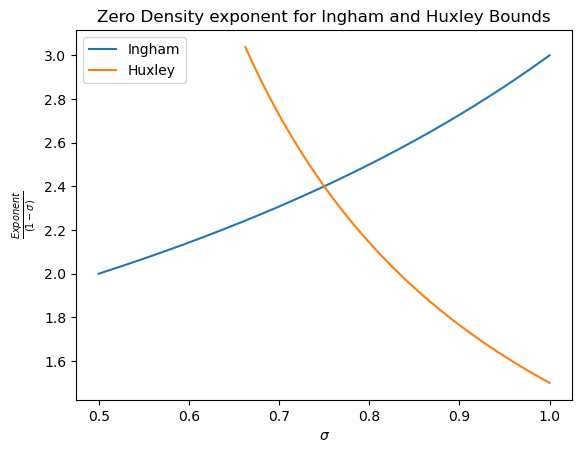
\includegraphics[width=\textwidth]{inghamhuxley2.png}
        \caption{$\sigma=3/4$ is also the bottleneck when written in Hoheisel's form.}
    \end{subfigure}
    \centering
    \begin{subfigure}{0.4\textwidth}
        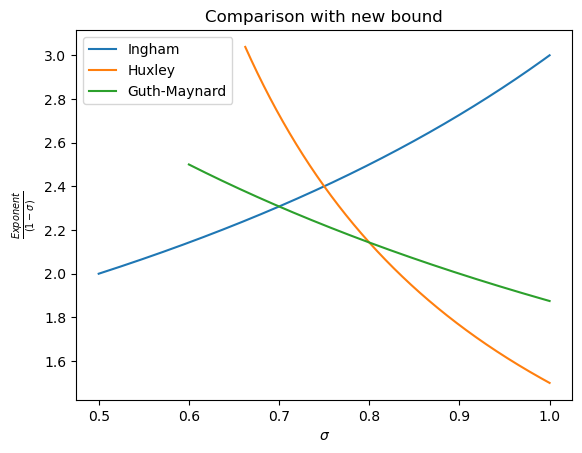
\includegraphics[width=\textwidth]{gm_2.png}
        \caption{The exponent is reduced around the bottleneck region.}
    \end{subfigure}
\end{figure}
\end{frame}

\begin{frame}{Idea of Zero density proof}
    \begin{enumerate}
        \item $\frac{1}{\zeta}(s)$ can be represented as \[
            \sum_{n} \frac{\mu(n)}{n^s}.
        \]
        \item Let $M_x(s)\defeq \sum_{n\leq x}\frac{\mu(n)}{n^s}$, which is an approximation of $1/\zeta$. Then we have by M\"obius inversion \[
        \zeta(s) M_x(s) = 1 + \sum_{n>x}a_{n,x}n^{-s}\approx 1 +\sum_{n>x}a_{n,x}n^{-s}e^{-n/y}\approx 1 +\sum_{y^2>n>x}a_{n,x}n^{-s}e^{-n/y}
        \]
        with some error decreasing in $y$.
        \item If $s$ is a zero of $\zeta$ then the left hand side is zero, which means the Dirichlet series on the right hand side has magnitude close to $1$.
    \end{enumerate}
\end{frame}
\section{Large Values Estimates results}
\begin{frame}{Guth-Maynard zero density result}
    \begin{theorem}[Guth-Maynard]
        Let $D_N(t) \defeq \sum_{N\leq x< 2N} b_n n^{i t}$. If $W\subset [0,T]$ is a set of $1$-separated points such that \[
        |D_N(t_i)|>V \ \forall t_i\in W
        \]
         then \[
         |W|\leq T^{o(1)}(\max_{N\leq n <2N} |b_n| )(N^2V^{-2} + N^{18/5}V^{-4}+TN^{12/5}V^{-4}).
         \]
    \end{theorem}

\end{frame}
\begin{frame}{Hybrid Zero Density and Dirichlet Value Estimate}
    There are generalizations for zero densities of Dirichlet-L functions $    L(s,\chi)\defeq\sum_{n} \chi(n)n^{-s}.$
    \begin{theorem}
        Let $D_N(t,\chi) \defeq \sum_{N\leq x< 2N} b_n\chi(n) n^{i t}$. If $W=\{t_i,\chi_i\}$ such that $\chi_i$ is a primitive character mod $q$, $t_i\in [0,T]$ are $1$-separated for the same character, \[
        |D_N(t_i,\chi_i)|>V \ \forall (t_i,\chi_i)\in W.
        \]
         Then we have for $N\geq q^{5/6}$ \[
         |W|\leq (qT)^{o(1)}(\max_{N\leq n <2N} |b_n| )(N^2V^{-2} + N^{18/5}V^{-4}+qTN^{12/5}V^{-4}).
         \]
    \end{theorem}
 
\end{frame}

\iffalse
\begin{frame}{References}
    \footnotesize
    \bibliography{project.bib}
    \bibliographystyle{abbrv}
\end{frame}
\fi
%------------------------------------------------
\iffalse
\begin{frame}{Blocks of Highlighted Text}
    In this slide, some important text will be \alert{highlighted} because it's important. Please, don't abuse it.

    \begin{block}{Block}
        Sample text
    \end{block}

    \begin{alertblock}{Alertblock}
        Sample text in red box
    \end{alertblock}

    \begin{examples}
        Sample text in green box. The title of the block is ``Examples".
    \end{examples}
\end{frame}

%------------------------------------------------

\begin{frame}{Multiple Columns}
    \begin{columns}[c] % The "c" option specifies centered vertical alignment while the "t" option is used for top vertical alignment

        \column{.45\textwidth} % Left column and width
        \textbf{Heading}
        \begin{enumerate}
            \item Statement
            \item Explanation
            \item Example
        \end{enumerate}

        \column{.45\textwidth} % Right column and width
        Lorem ipsum dolor sit amet, consectetur adipiscing elit. Integer lectus nisl, ultricies in feugiat rutrum, porttitor sit amet augue. Aliquam ut tortor mauris. Sed volutpat ante purus, quis accumsan dolor.

    \end{columns}
\end{frame}

%------------------------------------------------
\section{Second Section}
%------------------------------------------------

\begin{frame}{Table}
    \begin{table}
        \begin{tabular}{l l l}
            \toprule
            \textbf{Treatments} & \textbf{Response 1} & \textbf{Response 2} \\
            \midrule
            Treatment 1         & 0.0003262           & 0.562               \\
            Treatment 2         & 0.0015681           & 0.910               \\
            Treatment 3         & 0.0009271           & 0.296               \\
            \bottomrule
        \end{tabular}
        \caption{Table caption}
    \end{table}
\end{frame}

%------------------------------------------------

\begin{frame}{Theorem}
    \begin{theorem}[Mass--energy equivalence]
        $E = mc^2$
    \end{theorem}
\end{frame}

%------------------------------------------------

\begin{frame}{Figure}
    Uncomment the code on this slide to include your own image from the same directory as the template .TeX file.
    %\begin{figure}
    %\includegraphics[width=0.8\linewidth]{test}
    %\end{figure}
\end{frame}

%------------------------------------------------

\begin{frame}[fragile] % Need to use the fragile option when verbatim is used in the slide
    \frametitle{Citation}
    An example of the \verb|\cite| command to cite within the presentation:\\~

    This statement requires citation \cite{p1}.
\end{frame}

%------------------------------------------------

\begin{frame}{References}
    \footnotesize
    \bibliography{project.bib}
    %\bibliographystyle{apalike}
\end{frame}

%------------------------------------------------


%----------------------------------------------------------------------------------------
\fi
\end{document}